%   Rafael Corsi Ferrao
% 	corsiferrao@gmail.com / rafael.corsi@maua.br
%  		

\input{template}

\usepackage{lettrine}
\usepackage{enumitem}

%\usepackage[subsection]{placeins}


%\linespread{1.5} % Espaçamento de 1.5

% ------------------------------------------------------------------------
%\title { Introdução a FPGA \\ \vspace{5pt}	\normalfont \textit{Aula 1} }
%\author{ Rafael Corsi Ferrão }

\subject{BrasCubo}
\title{Manual de Montagem - Versão 1\\ CubeSat}
\author{Felipe Mahlmeister \\ \small \href{mailto:Felipe.Mahlmeister1@gmail.com}{Felipe.Mahlmeister1@gmail.com}}
%\date{}
\lowertitleback{}

% Footer
%\lfoot{\footnotesize Manual Montagem RWR - Mancal Magnético}

% ------------------------------------------------------------------------
\begin{document}

\maketitle
\tableofcontents

\section{Apresentação}

Neste documento será apresentado instruções de montagem do CubeSat, é recomendável a leitura prévia do  \textbf{\href{http://www.cubesat.org/images/developers/cds_rev13_final.pdf}{CubeSat Design Specification}} para conhecimento dos padrões internacionais a serem seguidos pelo projeto.

Estaremos exemplificando a princípio com um CubeSat 1U, e posteriormente com um CubeSat 3U, as especificações de dimensões estão descritas no documento acima nas sessões 01 e 04, respectivamente.


Os desenhos com dimensões das peças e as folhas de processos estão em um documento à parte: \textbf{Folhas de Processos}

A relação de número dos furos está na folha de processos.


\section{Peças}

Segue lista de peças que constituem o CubeSat 1U, assim como suas devidas quantidades:

\begin{itemize}
	\item \textbf{Cubesat-Struct-Ext-Shell-Side} : Casca externa lateral \textbf{(4 peças)}
	\item \textbf{Cubesat-Struct-Ext-Shell-Top} : Casca externa superior e inferior \textbf{(2 peças)}
	\item \textbf{Cubesat-Struct-Int-Frame-Side01} : Estrutura interna lateral principal \textbf{(2 peças)}
	\item \textbf{Cubesat-Struct-Int-Frame-Side02} : Estrutura interna lateral de ligação \textbf{(2 peças)}
	\item \textbf{Cubesat-Struct-Int-Frame-Side03} : Estrutura interna lateral de ligação \textbf{(2 peças)}
	\item \textbf{Cubesat-Struct-Int-Frame-Top} : Estrutura interna superior e inferior \textbf{(2 peças)}
	\item \textbf{Cubesat-Struct-Int-Plate-PCBStruct} : Placa de fixação entre a PCB e a estrutura (Frame-Side) \textbf{(4 peças)}
	\item \textbf{Cubesat-PCB-Side} : PCB lateral \textbf{(4 peças)}
	\item \textbf{Cubesat-PCB-Top} : PCB superior \textbf{(2 peças)}
\end{itemize}

\section{Ordem de montagem}

Para a montagem do \textbf{Conjunto01} (Figura \ref{1}, item 1.) será necessário alinhar os furos(01-04) entre a estrutura (Figura \ref{1-1},item 1.2.) e a placa (Figura \ref{1-2},item 1.3.), parafusar os quatro(04) parafusos (Figura \ref{1-3}, item 1.4.) juntamente com as quatro(04) porcas (Figura \ref{1-4}, item 1.6.), fixando assim a placa de fixação entre PCB e estrutura.

Para a fixação da PCB na placa por meio de parafusos, será necessário previamente soldar quatro(04) porcas (Figura \ref{1-5}, item 1.6.) nos furos(05-08).

A PCB (item 1.1.) deverá ser fixada na placa, por meio de parafusos (Figura \ref{1-6}, item 1.5.), finalizando assim a montagem do \textbf{Conjunto01}.

O \textbf{Conjunto02} trata-se da repetição dos procedimentos do \textbf{Conjunto01} (Figura \ref{2}, item 2.).

Para a montagem do \textbf{Conjunto03} será necessário posicionar a Estrutura interna lateral de ligação (Figura \ref{2}, item 2.)

\newpage

%Para a montagem do \textbf{Conjunto03}, começaremos posicionando e parafusando a Estrutura interna lateral de ligação na Estrutura interna lateral principal

%\begin{enumerate}
%	\item \textbf{Conjunto01}
%
%	\item \textbf{Conjunto02}
%	\begin{enumerate}[label*=\arabic*.]
%		\item Cubesat-PCB-Side \textbf{(01 peça)}
%		\item Cubesat-Struct-Int-Frame-Side01 \textbf{(01 peça)}
%		\item Cubesat-Struct-Int-Plate-PCBStruct \textbf{(01 peça)}
%		\item CubeSat-Toolbox-Int-Screw-M1.6-12mm \textbf{(04 peças)}
%		\item CubeSat-Toolbox-Int-Screw-M1.6-5mm \textbf{(04 peças)}
%		\item CubeSat-Toolbox-Int-Nut-M1.6 \textbf{(08 peças)}
%	\end{enumerate}
%	\item \textbf{Conjunto03}
%	\begin{enumerate}[label*=\arabic*.]
%		\item Cubesat-Struct-Int-Frame-Side02 \textbf{(01 peça)}
%		\item Cubesat-Struct-Int-Frame-Side03 \textbf{(01 peça)}
%	\end{enumerate}
%\end{enumerate}


% Conjunto 01

\subsection{Conjunto 01}\label{subs:c01}

O conjunto é formado pelas seguintes peças :

\begin{enumerate}[label*=\ref*{subs:c01}\arabic*]
	\item Cubesat-PCB-Side \textbf{(01 peça)}
	\item Cubesat-Struct-Int-Frame-Side01 \textbf{(01 peça)}
	\item Cubesat-Struct-Int-Plate-PCBStruct \textbf{(01 peça)}
	\item CubeSat-Toolbox-Int-Screw-M1.6-12mm \textbf{(04 peças)}
	\item CubeSat-Toolbox-Int-Screw-M1.6-5mm \textbf{(04 peças)}
	\item CubeSat-Toolbox-Int-Nut-M1.6 \textbf{(08 peças)}
\end{enumerate}

\begin{figure}[ht!]
	\centering
	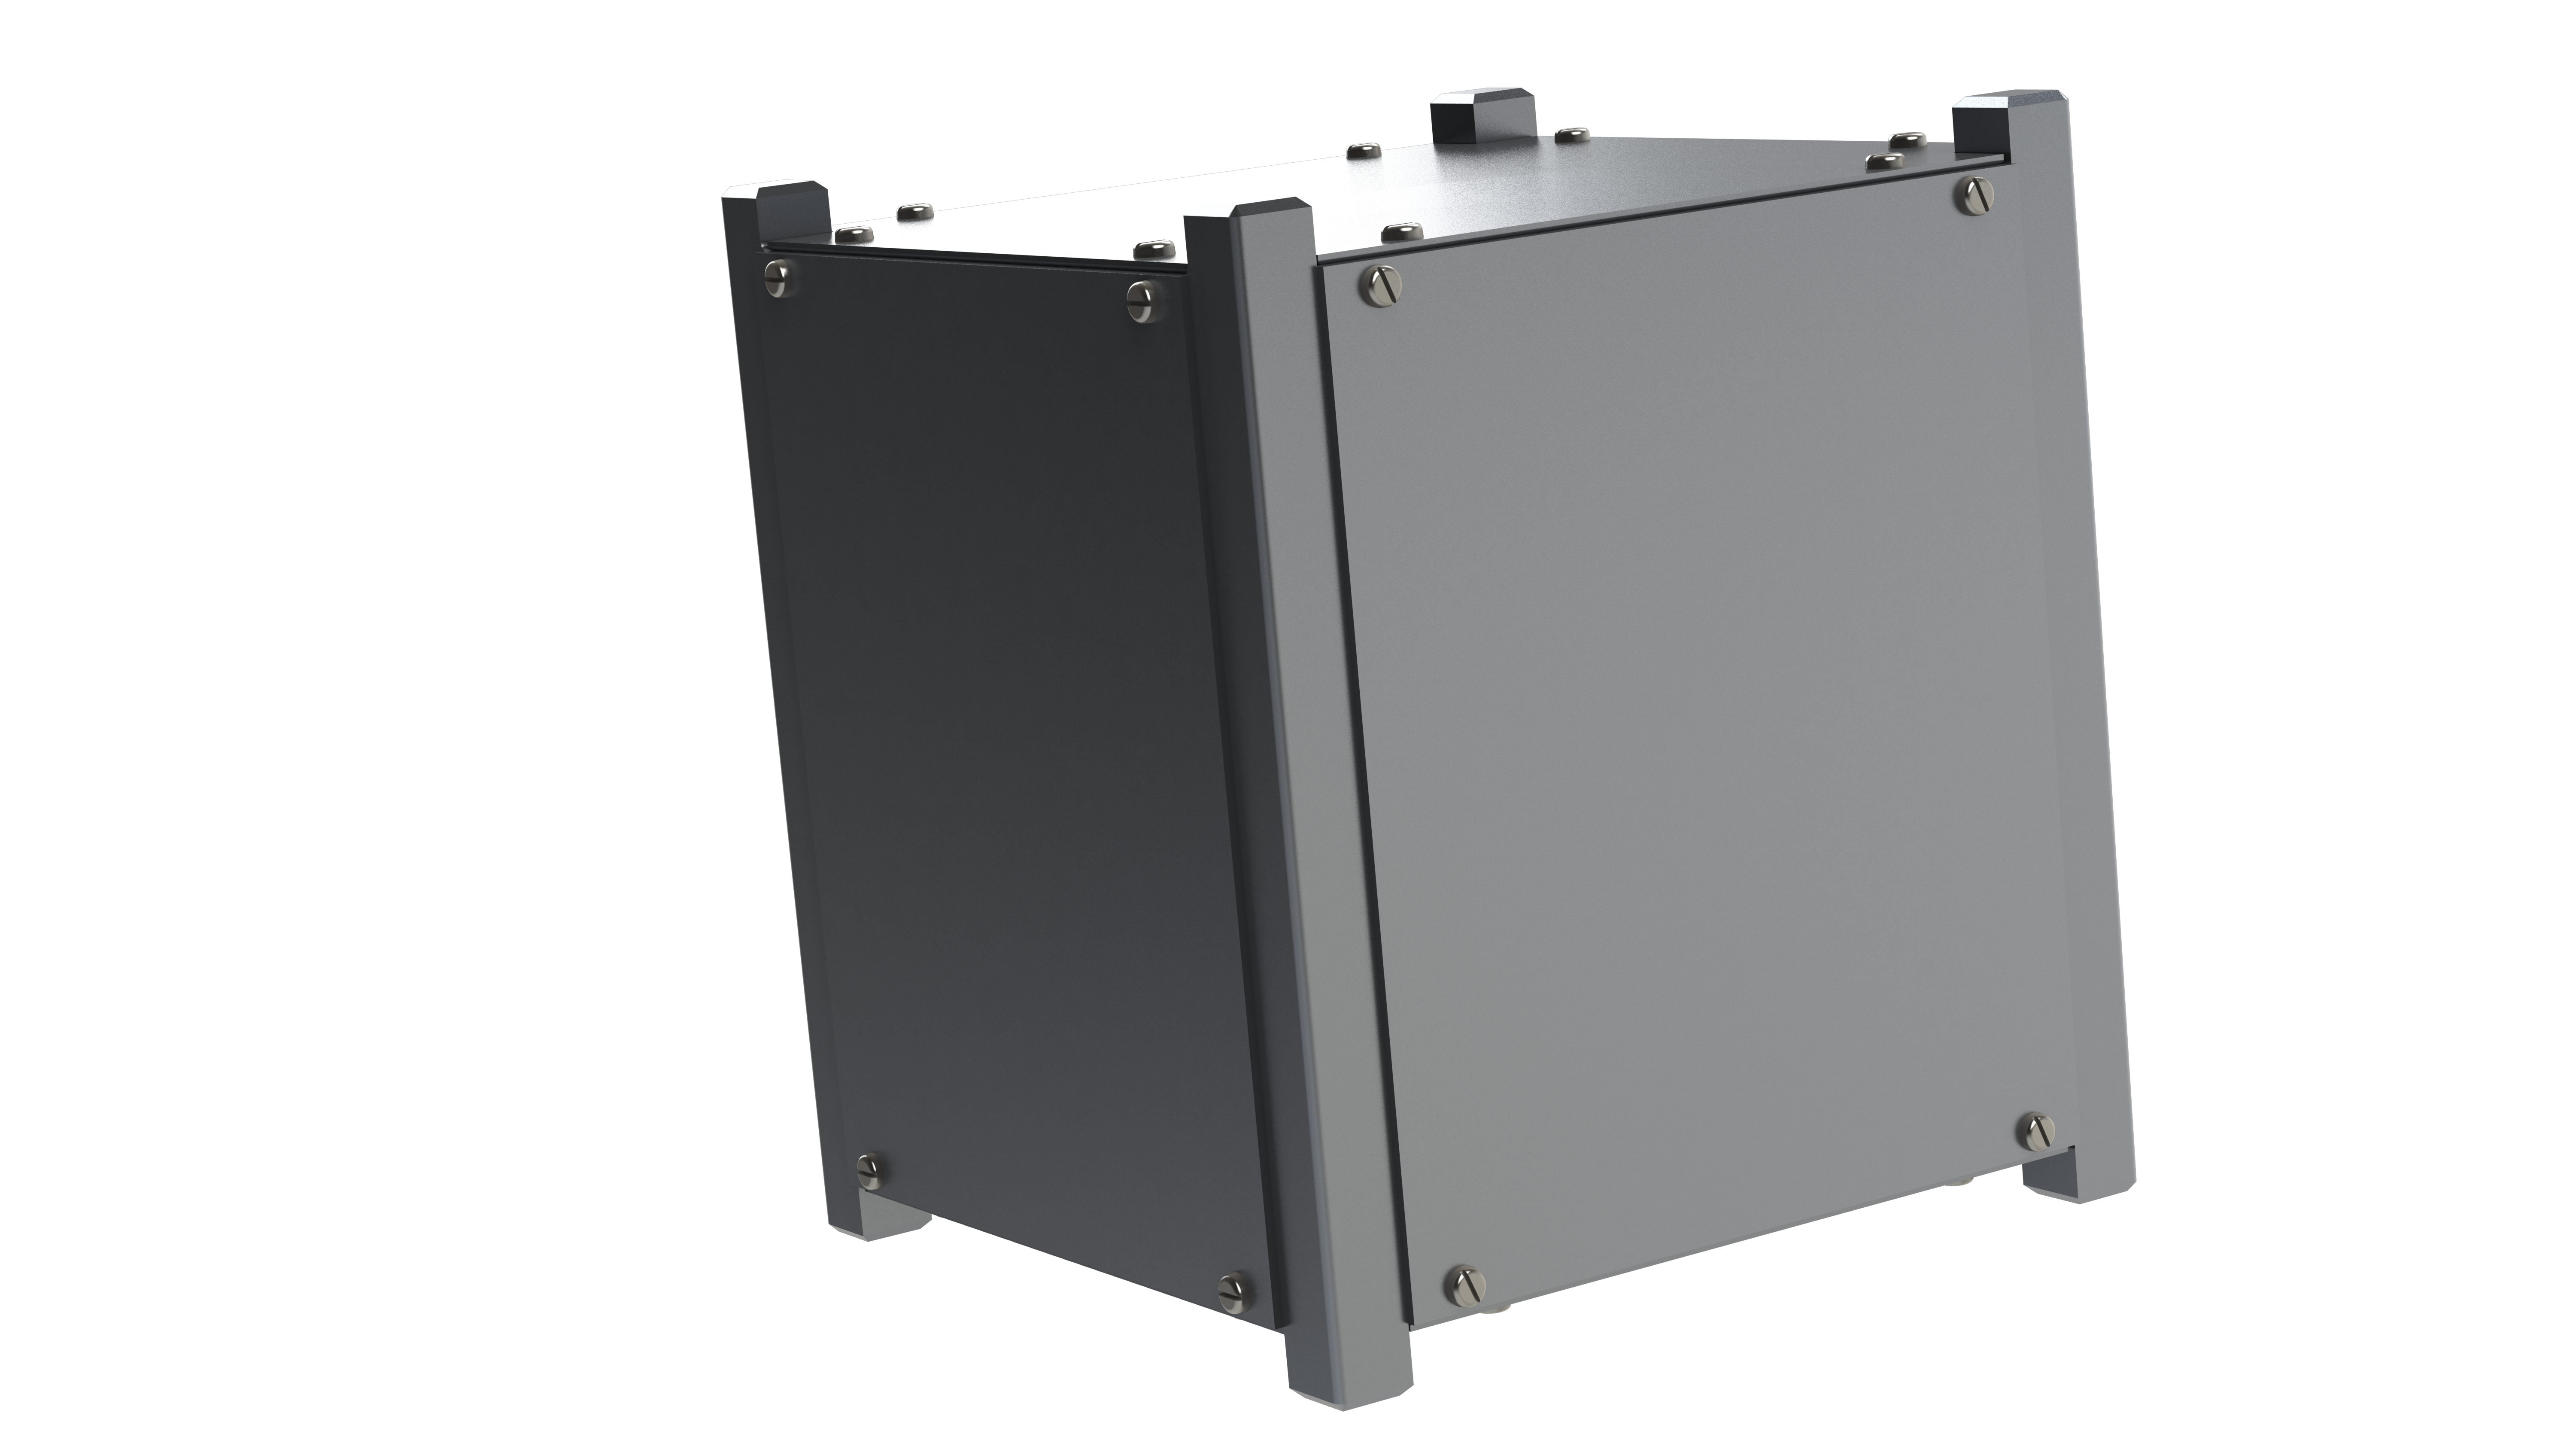
\includegraphics[width=0.8\textwidth]{img/1.png}
	\caption{Conjunto01}
	\label{1}
\end{figure}

\begin{figure}[ht!]
	\centering
	\includegraphics[width=0.8\textwidth]{img/1-1.png}
	\caption{Cubesat-Struct-Int-Frame-Side01}
	\label{1-1}
\end{figure}

\begin{figure}[ht!]
	\centering
	\includegraphics[width=0.5\textwidth]{img/1-2.png}
	\caption{Cubesat-Struct-Int-Plate-PCBStruct}
	\label{1-2}
\end{figure}

\begin{figure}[ht!]
	\centering
	\includegraphics[width=0.5\textwidth]{img/1-3.png}
	\caption{Fixação por parafuso da placa de fixação entre PCB e estrutura. furos(01-04)}
	\label{1-3}
\end{figure}

\begin{figure}[ht!]
	\centering
	\includegraphics[width=0.5\textwidth]{img/1-4.png}
	\caption{Fixação da porca para parafuso de fixação. furos(01-04)}
	\label{1-4}
\end{figure}

\begin{figure}[ht!]
	\centering
	\includegraphics[width=0.5\textwidth]{img/1-5.png}
	\caption{Porca soldada. furos(05-08)}
	\label{1-5}
\end{figure}

\begin{figure}[ht!]
	\centering
	\includegraphics[width=0.8\textwidth]{img/1-6.png}
	\caption{Fixação PCB com parafusos. furos(05-08)}
	\label{1-6}
\end{figure}


% Conjunto 02

\newpage
\subsection{Conjunto 02}\label{subs:c02}

\begin{enumerate}[label*=\ref*{subs:c02}\arabic*]
	\item Cubesat-PCB-Side \textbf{(01 peça)}
	\item Cubesat-Struct-Int-Frame-Side01 \textbf{(01 peça)}
	\item Cubesat-Struct-Int-Plate-PCBStruct \textbf{(01 peça)}
	\item CubeSat-Toolbox-Int-Screw-M1.6-12mm \textbf{(04 peças)}
	\item CubeSat-Toolbox-Int-Screw-M1.6-5mm \textbf{(04 peças)}
	\item CubeSat-Toolbox-Int-Nut-M1.6 \textbf{(08 peças)}
\end{enumerate}

\begin{figure}[ht!]
	\centering
	\includegraphics[width=0.8\textwidth]{img/2.png}
	\caption{Conjunto01}
	\label{2}
\end{figure}


% Conjunto 03

\newpage
\subsection{Conjunto 03}\label{subs:c03}

\begin{enumerate}[label*=\ref*{subs:c03}\arabic*]
	\item Cubesat-PCB-Side \textbf{(01 peça)}
	\item Cubesat-Struct-Int-Frame-Side01 \textbf{(01 peça)}
	\item Cubesat-Struct-Int-Plate-PCBStruct \textbf{(01 peça)}
	\item CubeSat-Toolbox-Int-Screw-M1.6-12mm \textbf{(04 peças)}
	\item CubeSat-Toolbox-Int-Screw-M1.6-5mm \textbf{(04 peças)}
	\item CubeSat-Toolbox-Int-Nut-M1.6 \textbf{(08 peças)}
\end{enumerate}

\begin{figure}[ht!]
	\centering
	\includegraphics[width=0.8\textwidth]{img/3.png}
	\caption{Conjunto01}
	\label{3}
\end{figure}

\begin{figure}[ht!]
	\centering
	\includegraphics[width=0.8\textwidth]{img/3-1.png}
	\caption{Conjunto01}
	\label{3-1}
\end{figure}

\begin{figure}[ht!]
	\centering
	\includegraphics[width=0.8\textwidth]{img/3-2.png}
	\caption{Conjunto01}
	\label{3-2}
\end{figure}

\begin{figure}[ht!]
	\centering
	\includegraphics[width=0.8\textwidth]{img/3-3.png}
	\caption{Conjunto01}
	\label{3-3}
\end{figure}

\begin{figure}[ht!]
	\centering
	\includegraphics[width=0.8\textwidth]{img/3-4.png}
	\caption{Conjunto01}
	\label{3-4}
\end{figure}

\begin{figure}[ht!]
	\centering
	\includegraphics[width=0.8\textwidth]{img/3-5.png}
	\caption{Conjunto01}
	\label{3-5}
\end{figure}

\begin{figure}[ht!]
	\centering
	\includegraphics[width=0.8\textwidth]{img/3-6.png}
	\caption{Conjunto01}
	\label{3-6}
\end{figure}

\begin{figure}[ht!]
	\centering
	\includegraphics[width=0.8\textwidth]{img/3-7.png}
	\caption{Conjunto01}
	\label{3-7}
\end{figure}

\begin{figure}[ht!]
	\centering
	\includegraphics[width=0.8\textwidth]{img/3-8.png}
	\caption{Conjunto01}
	\label{3-8}
\end{figure}

\begin{figure}[ht!]
	\centering
	\includegraphics[width=0.8\textwidth]{img/3-9.png}
	\caption{Conjunto01}
	\label{3-9}
\end{figure}


% Conjunto 04

\newpage
\subsection{Conjunto 04}\label{subs:c04}

\begin{enumerate}[label*=\ref*{subs:c04}\arabic*]
	\item Cubesat-PCB-Side \textbf{(01 peça)}
	\item Cubesat-Struct-Int-Frame-Side01 \textbf{(01 peça)}
	\item Cubesat-Struct-Int-Plate-PCBStruct \textbf{(01 peça)}
	\item CubeSat-Toolbox-Int-Screw-M1.6-12mm \textbf{(04 peças)}
	\item CubeSat-Toolbox-Int-Screw-M1.6-5mm \textbf{(04 peças)}
	\item CubeSat-Toolbox-Int-Nut-M1.6 \textbf{(08 peças)}
\end{enumerate}

\begin{figure}[ht!]
	\centering
	\includegraphics[width=0.8\textwidth]{img/4.png}
	\caption{Conjunto01}
	\label{4}
\end{figure}


% Conjunto 05

\newpage
\subsection{Conjunto 05}\label{subs:c05}

\begin{enumerate}[label*=\ref*{subs:c05}\arabic*]
	\item Cubesat-PCB-Side \textbf{(01 peça)}
	\item Cubesat-Struct-Int-Frame-Side01 \textbf{(01 peça)}
	\item Cubesat-Struct-Int-Plate-PCBStruct \textbf{(01 peça)}
	\item CubeSat-Toolbox-Int-Screw-M1.6-12mm \textbf{(04 peças)}
	\item CubeSat-Toolbox-Int-Screw-M1.6-5mm \textbf{(04 peças)}
	\item CubeSat-Toolbox-Int-Nut-M1.6 \textbf{(08 peças)}
\end{enumerate}

\begin{figure}[ht!]
	\centering
	\includegraphics[width=0.8\textwidth]{img/5.png}
	\caption{Conjunto01}
	\label{5}
\end{figure}

\begin{figure}[ht!]
	\centering
	\includegraphics[width=0.8\textwidth]{img/5-1.png}
	\caption{Conjunto01}
	\label{5-1}
\end{figure}

\begin{figure}[ht!]
	\centering
	\includegraphics[width=0.8\textwidth]{img/5-2.png}
	\caption{Conjunto01}
	\label{5-2}
\end{figure}

\begin{figure}[ht!]
	\centering
	\includegraphics[width=0.8\textwidth]{img/5-3.png}
	\caption{Conjunto01}
	\label{5-3}
\end{figure}

\begin{figure}[ht!]
	\centering
	\includegraphics[width=0.8\textwidth]{img/5-4.png}
	\caption{Conjunto01}
	\label{5-4}
\end{figure}

\begin{figure}[ht!]
	\centering
	\includegraphics[width=0.8\textwidth]{img/5-5.png}
	\caption{Conjunto01}
	\label{5-5}
\end{figure}

\begin{figure}[ht!]
	\centering
	\includegraphics[width=0.8\textwidth]{img/5-6.png}
	\caption{Conjunto01}
	\label{5-6}
\end{figure}


% Conjunto 06

\newpage
\subsection{Conjunto 06}\label{subs:c06}

\begin{enumerate}[label*=\ref*{subs:c06}\arabic*]
	\item Cubesat-PCB-Side \textbf{(01 peça)}
	\item Cubesat-Struct-Int-Frame-Side01 \textbf{(01 peça)}
	\item Cubesat-Struct-Int-Plate-PCBStruct \textbf{(01 peça)}
	\item CubeSat-Toolbox-Int-Screw-M1.6-12mm \textbf{(04 peças)}
	\item CubeSat-Toolbox-Int-Screw-M1.6-5mm \textbf{(04 peças)}
	\item CubeSat-Toolbox-Int-Nut-M1.6 \textbf{(08 peças)}
\end{enumerate}

\begin{figure}[ht!]
	\centering
	\includegraphics[width=0.8\textwidth]{img/6.png}
	\caption{Conjunto01}
	\label{6}
\end{figure}


% Conjunto 07

\newpage
\subsection{Conjunto 07}\label{subs:c07}

\begin{enumerate}[label*=\ref*{subs:c07}\arabic*]
	\item Cubesat-PCB-Side \textbf{(01 peça)}
	\item Cubesat-Struct-Int-Frame-Side01 \textbf{(01 peça)}
	\item Cubesat-Struct-Int-Plate-PCBStruct \textbf{(01 peça)}
	\item CubeSat-Toolbox-Int-Screw-M1.6-12mm \textbf{(04 peças)}
	\item CubeSat-Toolbox-Int-Screw-M1.6-5mm \textbf{(04 peças)}
	\item CubeSat-Toolbox-Int-Nut-M1.6 \textbf{(08 peças)}
\end{enumerate}

\begin{figure}[ht!]
	\centering
	\includegraphics[width=0.8\textwidth]{img/7.png}
	\caption{Conjunto01}
	\label{7}
\end{figure}


% Conjunto 08

\newpage
\subsection{Conjunto 08}\label{subs:c08}

\begin{enumerate}[label*=\ref*{subs:c08}\arabic*]
	\item Cubesat-PCB-Side \textbf{(01 peça)}
	\item Cubesat-Struct-Int-Frame-Side01 \textbf{(01 peça)}
	\item Cubesat-Struct-Int-Plate-PCBStruct \textbf{(01 peça)}
	\item CubeSat-Toolbox-Int-Screw-M1.6-12mm \textbf{(04 peças)}
	\item CubeSat-Toolbox-Int-Screw-M1.6-5mm \textbf{(04 peças)}
	\item CubeSat-Toolbox-Int-Nut-M1.6 \textbf{(08 peças)}
\end{enumerate}

\begin{figure}[ht!]
	\centering
	\includegraphics[width=0.8\textwidth]{img/8.png}
	\caption{Conjunto01}
	\label{8}
\end{figure}

\begin{figure}[ht!]
	\centering
	\includegraphics[width=0.8\textwidth]{img/8-1.png}
	\caption{Conjunto01}
	\label{8-1}
\end{figure}

\begin{figure}[ht!]
	\centering
	\includegraphics[width=0.8\textwidth]{img/8-2.png}
	\caption{Conjunto01}
	\label{8-2}
\end{figure}

\begin{figure}[ht!]
	\centering
	\includegraphics[width=0.8\textwidth]{img/8-3.png}
	\caption{Conjunto01}
	\label{8-3}
\end{figure}

\begin{figure}[ht!]
	\centering
	\includegraphics[width=0.8\textwidth]{img/8-4.png}
	\caption{Conjunto01}
	\label{8-4}
\end{figure}


% Conjunto 09

\newpage
\subsection{Conjunto 09}\label{subs:c09}

\begin{enumerate}[label*=\ref*{subs:c09}\arabic*]
	\item Cubesat-PCB-Side \textbf{(01 peça)}
	\item Cubesat-Struct-Int-Frame-Side01 \textbf{(01 peça)}
	\item Cubesat-Struct-Int-Plate-PCBStruct \textbf{(01 peça)}
	\item CubeSat-Toolbox-Int-Screw-M1.6-12mm \textbf{(04 peças)}
	\item CubeSat-Toolbox-Int-Screw-M1.6-5mm \textbf{(04 peças)}
	\item CubeSat-Toolbox-Int-Nut-M1.6 \textbf{(08 peças)}
\end{enumerate}

\begin{figure}[ht!]
	\centering
	\includegraphics[width=0.8\textwidth]{img/9-1.png}
	\caption{Conjunto01}
	\label{9-1}
\end{figure}

\begin{figure}[ht!]
	\centering
	\includegraphics[width=0.8\textwidth]{img/9-2.png}
	\caption{Conjunto01}
	\label{9-2}
\end{figure}

\begin{figure}[ht!]
	\centering
	\includegraphics[width=0.8\textwidth]{img/9-3.png}
	\caption{Conjunto01}
	\label{9-3}
\end{figure}


% Conjunto 10

\newpage
\subsection{Conjunto 10}\label{subs:c10}

\begin{enumerate}[label*=\ref*{subs:c10}\arabic*]
	\item Cubesat-PCB-Side \textbf{(01 peça)}
	\item Cubesat-Struct-Int-Frame-Side01 \textbf{(01 peça)}
	\item Cubesat-Struct-Int-Plate-PCBStruct \textbf{(01 peça)}
	\item CubeSat-Toolbox-Int-Screw-M1.6-12mm \textbf{(04 peças)}
	\item CubeSat-Toolbox-Int-Screw-M1.6-5mm \textbf{(04 peças)}
	\item CubeSat-Toolbox-Int-Nut-M1.6 \textbf{(08 peças)}
\end{enumerate}

\begin{figure}[ht!]
	\centering
	\includegraphics[width=0.8\textwidth]{img/10.png}
	\caption{Conjunto01}
	\label{10}
\end{figure}










%%
%
%\begin{figure}
%	\centering
%	\includegraphics[width=\textwidth]{img/2.png}
%	\caption{Conjunto02}
%	\label{2}
%\end{figure}
%
%
%%Conjunto03
%
%\begin{figure}
%	\centering
%	\includegraphics[width=\textwidth]{img/3-1.png}
%	\caption{Cubesat-Struct-Int-Frame-Side02}
%	\label{3-1}
%\end{figure}
%
%\begin{figure}
%	\centering
%	\includegraphics[width=\textwidth]{img/3-2.png}
%	\caption{Cubesat-Struct-Int-Frame-Side03}
%	\label{3-2}
%\end{figure}
%
%
%
%%\section{Anexo partes}
%%\begin{table}
%%\centering
%%	\begin{tabular}{l c l}
%%		Ref  	& Qty & Descrição \\ 
%%		\hline
%%		RW-M-BA	 & 01 & Base do mancal \\
%%		RW-M-C	 & 01 & Casca externa \\
%%		RW-M-EEB & 01 & Estator externo base \\
%%		RW-M-EET & 01 & Estator externo topo \\
%%		RW-M-BT  & 01 & Batente \\
%%		RW-M-RFB & 01 & Rotor ferro base \\
%%		RW-M-RFT & 01 & Rotor ferro topo \\
%%		RW-M-RN	 & 01 & Rotor núcleo \\
%%		RW-M-EI	 & 01 & Estator interno \\
%%		RM-M-MAG & 11 & Imãs \\
%%		RM-M-EL	 & 01 & Eletrônica		
%%	\end{tabular} 
%%\end{table}
%


% ------------------------------------------------------------------------
\end{document}
% ------------------------------------------------------------------------


%\begin{figure}[ht!]  
%	\centering
%		\includegraphics[width=0.6 \columnwidth,angle=0]{figs/svpwm.pdf}
%	\caption{Acionamento SVPWM}
%	\label{fig:svpwm}
%\end{figure}